\chapter[SCP-137 真实玩具]{
    SCP-137 The Real Toy\\
    SCP-137 真实玩具
}

\label{chap:SCP-137}

\begin{figure}[H]
    \centering
    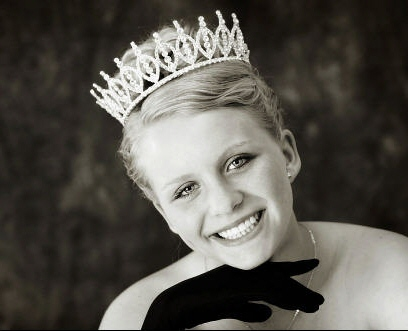
\includegraphics[width=0.5\linewidth]{images/SCP.137.jpg}
    \caption*{SCP-137目前的形态。}
\end{figure}

\bb{项目编号:}SCP-137

\bb{项目等级:}Euclid

\bb{特殊收容措施:}SCP-137应被安置在一个上锁的房间内,并提供一把梳子和一张绘有乡村草原的海报,以保持对象的温和与驯服。应向SCP-137提供一日三餐。任何情况下不允许将任何玩具带到SCP-137周围500米范围内。

\bb{描述:}SCP-137是一个能操纵玩具的个体,它能赋予玩具其本身所代表的东西的物理性质、大小和形状。举例来说,一只泰迪熊会变成一只真熊,并作出相应的行为。SCP-137无法操纵玩具以外的其他任何对象。观测到SCP-137能操纵物体的距离是250米,但直到进一步实验完成之前,假定其能力的最大作用范围是500米。

SCP-137首次引起基金会注意是在一连串涉及到儿童的意外死亡事件和意外后。对于一个连环杀手来说这些杀人事件显得过于没有规律,因此基金会特工被派遣调查。在采访了一个患有创伤后应激障碍的女孩之后(一个裸男突然出现在她的卧室),确认了此SCP的存在。在同一个街区与其再次遭遇时其呈现一只猩猩的形态。SCP-137被追踪,且在其于█████,████占据了一只小马玩具娃娃并被追赶至最近的荒野后最终被捕获。SCP-137被实施了镇定措施并由直升机送往19区。

实验证明SCP-137能呈现出被其操纵的玩具的特性,但只有孩子能察觉到。一个玩具士兵会变成一个暴力的,全副武装的男人。一把玩具枪能射出子弹。一只玩具狮子会攻击和杀死人类。然而,它缺乏真正的智能。它没有表现出有长期记忆的迹象,也缺乏任何的学习能力和抽象思考能力(见采访137-1)。更多资料请看\hyperref[sec:DOC-experiment-log-137]{实验日志137}。

对象通常栖身于一个████████ ██████线的公主娃娃。

\bb{附录}\\
\bb{采访137-1:}

\bb{被采访:}SCP-137

\bb{采访者:}█████博士

\bb{前言:}进行采访是为了弄清SCP-137是什么,以及它为何\slash 如何操纵玩具。

\bb{<日志开始>}

\ii{█████博士:}日安。

\ii{SCP-137:}你好呀!我是Blossom公主。你是我的王子吗?

\ii{█████博士:}不。现在,能请你告诉我你是什么吗?

\ii{SCP-137:}我是个公主!我是全世界最美丽的公主!

\ii{█████博士:}你来自哪里?

\ii{SCP-137:}我住在一个城堡里。你是我的王子吗?

*进一步的询问得到了相似的结果。*

\bb{<日志结束>}

\newpage
\section{实验日志137}

\label{sec:DOC-experiment-log-137}

\begin{scpbox}

\bb{日期:}██\slash ██\slash ████\\
\bb{测试对象:}玩具飞机

\ii{结果:}玩具变成一架实物大小的F-16,该飞机试图在实验设施内起飞并造成大量破坏。其残骸迅速变回塑料,而SCP-137复原为目前的形态。

\ii{备忘:}将来请避免测试配备有喷气发动机和导弹的物品。这是个昂贵的实验。

\end{scpbox}

\begin{scpbox}

\bb{日期:}██\slash ██\slash ████\\
\bb{测试对象:}███ ██████ 牌子的赛车

\ii{结果:}玩具变成一辆实物大小的法拉利,试图在实验设施内到处行驶并最终高速撞上墙壁。与上次一样,其残骸迅速变回塑料而SCP-137复原为目前的形态。

\ii{备忘:}车辆实验现在需要得到 ████████主管的安全许可。

\end{scpbox}

\begin{scpbox}

\bb{日期:}██\slash ██\slash ████\\
\bb{测试对象:}一个扣在特工Sorenson的钥匙上的美洲鳄钥匙扣

\ii{结果:}一只六米长的咸水鳄出现在走廊。十四人死亡。

\ii{备忘:}所有特工在进入██号地点之前都必须被搜走身上的玩具或者像玩具的物品。

\end{scpbox}

\begin{scpbox}

\bb{日期:}██\slash ██\slash ████\\
\bb{测试对象:}█████ 牌子的“美国士兵”可动人形

\ii{结果:}玩具变成一个穿着士兵制服,携带一把大型步枪的成年男性。在被消灭之前该男性设法杀害了五名工作人员。

\ii{备忘:}下次试试不这么暴力的东西吧。

\end{scpbox}

\begin{scpbox}

\bb{日期:}██\slash ██\slash ████\\
\bb{测试对象:}██████ 牌子的“巡警囧死”(Officer Jones beat cop)可动人形

\ii{结果:}一个穿着警察制服的成年男性。它不停询问“犯人”去了哪里,并且坚称研究人员们禁止携带违禁药品。他试图审讯研究人员,并宣称研究人员们是罪犯,且在被消灭之前射击了两人,逮捕了第三个研究人员。

\end{scpbox}

\begin{scpbox}

\bb{日期:}██\slash ██\slash ████\\
\bb{测试对象:}一只胖熊猫

\ii{结果:}一只非常大的熊猫。需要注意的是,尽管它们有着“可爱”的外表和食草动物的习性,但熊猫仍然是熊。它抱住了研究人员之一,并在被消灭之前折断了其三根肋骨。

\end{scpbox}

\begin{scpbox}

\bb{日期:}██\slash ██\slash ████\\
\bb{测试对象:}一盒 ████ 塑料积木

\ii{结果:}一块陶砖出现在盒子里。随后它消失了,被另一块不同材质的板砖取代。这个现象持续了数小时,直到被摧毁。之后SCP-137重新激活了目前的寄主。

\end{scpbox}

\begin{scpbox}

\bb{日期:}██\slash ██\slash ████\\
\bb{测试对象:}一个███████ 牌子的溜溜球

\ii{结果:}溜溜球没有改变形态。但是,它变得拥有自主性,开始自己移动和作出各种花式,甚至被从研究人员的手指上拿下来或被挂在墙上时也一样。

\end{scpbox}

\begin{scpbox}

\bb{日期:}██\slash ██\slash ████\\
\bb{测试对象:}一个██████ 牌子的Selenium博士玩具人,包装上写着“世界上最聪明的人”

\ii{结果:}一个穿着实验外套的成年男性。它反复提到自己有“惊人的智力”。但是,当问及任何科学或数学知识时,它不会直接回答,而只是说自己是“世界上最聪明的人”。在数个小时徒劳的提问之后实验结束。

\end{scpbox}

